% 页面设置
\documentclass[12pt, a4paper]{article} % 字号:12,纸张:A4
\usepackage[top=2.54cm, bottom=2.54cm, left=3.18cm,right=3.18cm]{geometry} % 页边距设置
% 字体设置
\usepackage[UTF8]{ctex}
\usepackage{fontspec} % 设置字体
%\setCJKmainfont{SimSun}[AutoFakeBold=true, BoldFont={SimHei}, ItalicFont={KaiTi}] % 正文字体
%\setCJKsansfont[AutoFakeBold=3]{KaiTi} % 无衬线字体
%\setCJKmonofont[AutoFakeBold=3]{SimHei} % 等宽字体
\setmainfont{Times New Roman} % 设置主字体为新罗马体
% 文本设置
\usepackage{enumerate} % 支持小标题编号
\linespread{1.5} % 行间距1.5倍
\usepackage{indentfirst}%首段缩进
\setlength{\parindent}{2em} % 首行缩进两字符
\usepackage[hidelinks]{hyperref} % 目录添加超链接
\usepackage{zhnumber} % 章节标题中文显示
\usepackage[cmyk]{xcolor} % 文字彩色显示
% 数学支持
\usepackage{amsmath} % 数学公式支持
\usepackage{amssymb} % 数学符号支持
\usepackage{bm} % 公式加粗
\usepackage{mathrsfs} % 花体字母
\usepackage{yhmath} % 更多的数学符号
% 图片设置
\usepackage{caption} % 插入图片标题
\usepackage{float} % 控制图片位置
\usepackage{subfigure} % 图片并排
\usepackage{booktabs} % 插入表格
% 表格设置
\usepackage{multirow} % 表格自动换行
\usepackage{bigstrut} % 表格间距
\usepackage{rotating} % 表格旋转
\usepackage{tabularx} % 表格宽度
\usepackage{colortbl} % 表格颜色
\usepackage{graphicx} % 表格自动宽度

\title{第七章 \ \ \ 贝叶斯分类器} % 文章标题
\author{Castor Ye} % 文章作者
\date{} % 文章时间

\begin{document} % 文档从这里开始。
\maketitle % 按照预定的模板把上面那些信息排好。
\newtheorem{definition}{定义}[section]
\newtheorem{theorem}{定理}[section]
\newtheorem{example}{例}[section]
\newtheorem{solution}{题解}
\newtheorem{algorithm}{算法}
\newtheorem{axiom}{公理}
\newtheorem{property}{性质}
\newtheorem{proposition}{命题}
\newtheorem{lemma}{引理}
\newtheorem{corollary}{推论}[section]
\newtheorem{remark}{注解}
\newtheorem{condition}{条件}
\newtheorem{conclusion}{结论}
\newtheorem{assumption}{假设}
\renewcommand{\figurename}{图} % 将图片序号改为图
\renewcommand{\tablename}{表} % 将表格序号改为表
%%%%%%%%%%%%%%%%%%%%%%%%%%%%%%%%%%%%%%%%%%%%%%%%%%%%%%%%%%%%%%%%%%%%%%%
% 文章内容从此开始
贝叶斯分类器是一种概率框架下的统计学习分类器,对分类任务而言,假设在相关概率都已知的情况下,贝叶斯分类器考虑如何基于这些概率为样本判定最优的类标。

\begin{theorem}
    设试验 $E$ 的样本空间为 $S$,$A$ 为 $E$ 的事件,$B_1, B_2, \cdots, B_n$ 为 $S$ 的一个划分,且 $P(A) > 0, P(B_i) > 0 \ \ \ (i = 1, 2, \cdots, n)$,则有贝叶斯公式:
    \begin{equation*}
        P(B_i | A) = \frac{P(A|B_i) P(B_i)}{\displaystyle \sum_{j = 1}^{n} P(A | B_j) P(B_j)}, i = 1, 2, \cdots, n
    \end{equation*} 
\end{theorem}

\section{贝叶斯决策论}

假设有 $N$ 种可能的类别标记,即 $Y = \{c_1, c_2, \cdots, c_N\}$,$\lambda_{ij}$ 是将一个真实标记为 $c_j$ 的样本误分类为 $c_i$ 所产生的损失。基于后验概率 $P(c_i | x)$ 可获得将样本 $x$ 分类为 $c_i$ 所产生的期望损失(expected loss),即在样本 $x$ 上的“条件风险”(conditional risk):
\begin{equation*}
    R(c_i | x) = \sum_{j = 1}^{N} \lambda_{ij} P(c_j | x)
\end{equation*}

我们的任务是寻找一个判定准则 $h: X \to Y$ 以最小化总体风险:
\begin{equation*}
    R(h) = \mathbb{E}_{x} [R(h(x) | x)]
\end{equation*}
显然,对每个样本 $x$,若 $h$ 能最小化条件风险 $R(h(x) | x)$,则总体风险 $R(h)$ 也将最小化。这就产生了贝叶斯判定准则(Bayes decision rule):为最小化总体风险,只需在每个样本上选择那个能使条件风险 $R(c | x)$ 最小的类别标记。即:
\begin{equation*}
    h^* (x) = arg \min_{c \in Y} R(c | x)
\end{equation*}
此时,$h^*$ 称为贝叶斯最优分类器(Bayes optimal classifier),与之对应的总体风险 $R(h^*)$ 称为贝叶斯风险(Bayes risk)。$1 - R(h^*)$ 反映了分类其所能达到的最好性能,即通过机器学习所能产生的模型精度的理论上限。

具体来说,若 $\lambda_{ij}$ 取 $0-1$ 损失,则有:
\begin{equation*}
    R(c | x) = 1 - P(c | x), \ \ \ h^* (x) = arg \max_{c \in Y} P(c | x)
\end{equation*}
即对每个样本 $x$,选择能使后验概率 $P(c | x)$ 最大的类别标记。

一般情况有两种策略来对后验概率进行估计:
\begin{enumerate}[\hspace*{2em} i.]
    \item 判别式模型:直接对 $P(c | x)$ 进行建模求解,例如前面的决策树、神经网络、svm。
    \item 生成式模型:通过先对联合分布 $P(x, c)$ 建模,从而进一步求解 $P(c | x)$。
\end{enumerate}

贝叶斯分类器和属于生成式模型,必然考虑:
\begin{equation*}
    P(c | x) = \frac{P(x, c)}{P(x)}
\end{equation*}
基于贝叶斯定理,$P(c | x)$ 可写为:
\begin{equation*}
    P(c | x) = \frac{P(c) P(x | c)}{P(x)}
\end{equation*}
其中,$P(c)$ 是类“先验”(prior)概率;$P(x | c)$ 是样本 $x$ 相对于类标记 $c$ 的类条件概率(class-conditional probability),或称为“似然”(likelihood);$P(x)$ 是用于归一化的“证据”(evidence)因子。

对于类先验概率 $P(c)$,$P (c)$ 就是样本空间中各类样本所占的比例,根据大数定理(当样本足够多时,频率趋于稳定等于其概率),这样当训练样本充足时,$P(c)$ 可以使用各类出现的频率来代替。因此只剩下类条件概率 $P(x | c)$,它表达的意思是在类别c中出现x的概率,它涉及到属性的联合概率问题,若只有一个离散属性还好,当属性多时采用频率估计起来就十分困难,因此这里一般采用极大似然法进行估计。

\section{极大似然法}

极大似然估计(Maximum Likelihood Estimation, MLE)是根据数据采样类估计概率分布的经典方法,常用的策略是先假定总体具有某种确定的概率分布,再基于训练样本对概率分布的参数进行估计。

令 $D_c$ 表示训练集 $D$ 中第 $c$ 类样本组成的集合,假设这些样本是独立同分布的,则参数 $\theta_c$ 对于数据集 $D_c$ 的似然是:
\begin{equation*}
    P(D_c | \theta_c) = \Pi_{x \in D_c} P(x | \theta_c)
\end{equation*}
对 $\theta_c$ 进行极大似然估计,就是去寻找能最大化似然 $P(D_c | \theta_c)$ 的参数值 $\hat{\theta}_c$。直观上看,极大似然估计是试图在 $\theta_c$ 所有可能的取值中,找到一个能使数据出现“可能性”最大的值。

\section{朴素贝叶斯分类器}

不难看出:原始的贝叶斯分类器最大的问题在于联合概率密度函数的估计,首先需要根据经验来假设联合概率分布,其次当属性很多时,训练样本往往覆盖不够,参数的估计会出现很大的偏差。为了避免这个问题,朴素贝叶斯分类器(naive Bayes classifier)采用了“属性条件独立性假设”,即样本数据的所有属性之间相互独立。这样类条件概率 $P(x | c)$ 可以改写为:
\begin{equation*}
    P(x | c) = \Pi_{i = 1}^{d} P(x_i | c)
\end{equation*}
其中 $d$ 为属性数目,$x_i$ 为 $x$ 在第 $i$ 个属性上的值。

由于对所有类别来说 $P(x)$ 相同,因此有朴素贝叶斯分类器表达式:
\begin{equation*}
    h_{nb}(x) = arg \max_{c \in Y} P(c) \Pi_{i = 1}^{d} P(x_i | c)
\end{equation*}

这样,为每个样本估计类条件概率变成为每个样本的每个属性估计类条件概率。

\begin{enumerate}[\hspace*{2em} i.]
    \item 离散属性,属性的类条件概率可估计为:
    \begin{equation*}
        P(x_i | c) = \frac{|D_{c, x_i}|}{|D_c|}
    \end{equation*}
    \item 连续属性,若假设属性服从正态分布,则属性的类条件概率可估计为:
    \begin{equation*}
        p(x_i | c) = \frac{1}{\sqrt{2 \pi} \sigma_{c, i}} \exp (- \frac{(x_i - \mu_{c, i})^2}{2 \sigma_{c, i}^{2}})
    \end{equation*}
\end{enumerate}

为了避免其他属性携带的信息被训练集中未出现的属性值“抹去”,在估计概率值是通常要进行“平滑”(smoothing),常用“拉普拉斯修正”(Laplacian correction)。具体来说,令 $N$ 表示训练集 $D$ 中可能的类别数,$N_i$ 表示第 $i$ 个属性可能的取值数,则有:
\begin{equation*}
    \hat{P}(c) = \frac{|D_c| + 1}{|D| + N}, \ \ \ \hat{P}(x_i | c) = \frac{|D_{c, x_i}| + 1}{|D_c| + N_i}
\end{equation*}

\section{半朴素贝叶斯}

为了降低贝叶斯公式中估计后验概率 $P(c | x)$ 的困难,朴素贝叶斯采用了属性条件独立性假设,但在现实任务中这个假设往往很难成立。于是,人们尝试对属性条件独立性假设进行一定程度的放松,由此产生了一类为“半朴素贝叶斯分类器”(semi-naive Bayes classifiers)的学习方法。

半朴素贝叶斯分类器的基本想法是适当考虑一部分属性间的相互依赖信息,从而概不需要进行为完全联合概率计算,又不至于彻底忽略了比较强的属性依赖关系。“独依赖估计”(One-Dependent Estimater, ODE)是朴素贝叶斯分类器最常用的一种策略。所谓“独依赖”就是假设每个属性在类别之外最多仅依赖于一个其他属性,即:
\begin{equation*}
    \displaystyle P(c | x) \propto P(c) \displaystyle \prod_{i = 1}^{d} P(x_i + c, pa_i)
\end{equation*}
其中 $pa_i$ 为属性 $x_i$ 所依赖的属性,称为 $x_i$ 的父属性。此时,对每个属性 $x_i$,若其父属性 $pa_i$ 已知,则可估计概率值 $P(x_i | c, pa_i)$。于是,问题的关键就转化为如何确定每个属性的父属性,不同的做法产生不同的独依赖分类器。

最直接的做法是假设所有属性都依赖于同一个属性,称为“超父”(super-parent),然后通过交叉验证等模型选择方法来确定超父属性,由此形成了 SPODE(Super-Parent ODE)方法。

\begin{figure}[H]
    \centering
    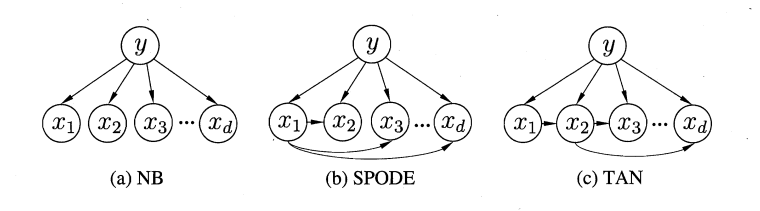
\includegraphics[width=0.8\textwidth]{../img/7-1-朴素贝叶斯与两种半朴素贝叶斯分类器所考虑的属性依赖关系.png}
    \caption{朴素贝叶斯与两种半朴素贝叶斯分类器所考虑的属性依赖关系}
    \label{fig:朴素贝叶斯与两种半朴素贝叶斯分类器所考虑的属性依赖关系}
\end{figure}

TAN(Tree Augmented naive Bayes)则是在最大带权生成树(maximum weighted spanning tree)算法的基础上,通过以下步骤将属性间依赖关系约简为图 \ref{fig:朴素贝叶斯与两种半朴素贝叶斯分类器所考虑的属性依赖关系} 所示的树形结构:

\begin{enumerate}[\hspace*{2em} i.]
    \item 计算任意两个属性之间的条件互信息(conditional mutual information):
    \begin{equation*}
        I(x_i, x_j | y) = \sum_{x_i, x_j; c \in Y} P(x_i, x_j | c) \log \frac{P(x_i, x_j | c)}{P(x_i | c)P(x_j | c)}
    \end{equation*}
    \item 以属性为结点构建完全图,任意两个结点之间边的权重设为 $I(x_i, x_j | y)$。
    \item 构建此完全图的最大带权生成树,挑选根变量,将边置为有向。
    \item 加入类别结点 $y$,增加从 $y$ 到每个属性的有向边。
\end{enumerate}

容易看出,条件互信息 $I(x_i, x_j | y)$ 刻画了属性 $x_i$ 和 $x_j$ 在已知类别情况下的相关性。

AODE(Averaged One-Dependent Estimator)是一种基于集成学习机制、更为强大的独依赖分类器。与 SPODE 通过模型选择确定超父属性不同,AODE 尝试将每个属性作为超父来构建 SPODE,然后将那些具有足够训练数据支撑的 SPODE 集成起来作为最终结果,即:
\begin{equation*}
    P(c | x) \propto \sum_{i = 1, |D_{x_i}| \ge m^{\prime}}^{d} P(c, x_i) \prod_{j = 1}^{d} P(x_j | c, x_i)
\end{equation*}
其中 $D_{x_i}$ 是在第 $i$ 个属性上取值为 $x_i$ 的样本的集合,$m^\prime$ 为阈值常数。显然,AODE 需估计 $P(c, x_i)$ 和 $P(x_j | c, x_i)$。

\section{EM 算法}




\end{document}